\chapter*{Introduction générale}
\newpage
\pagestyle{fancy}
\fancyhead[L]{}
\fancyhead[R]{Introduction générale}
\renewcommand{\headrulewidth}{1pt}
\fancyfoot[C]{\thepage}


\section*{Introduction}
La détection d'objets, comme étape principale dans n'importe quel processus  de reconnaissance, est la procédure consistant à déterminer l'instance de la classe à laquelle appartient l'objet et à estimer l'emplacement de l'objet en affichant le cadre de délimitation autour de l'objet. La détection d'une instance unique de classe à partir d'une image est appelée détection d'objet à classe unique, tandis que la détection des classes de tous les objets présents dans l'image est connue sous le nom de détection d'objet multi-classes. 

Récemment, la détection d'objets basée sur l'apprentissage profond a atteint de très bonnes performances. Cependant, il existe de nombreux défis avec les images prises dans le monde réel, tels que le bruit, l'occlusion partielle/complète, les conditions d'éclairage, la rotation, etc. Ces problèmes ont un impact important sur la détection des objets et doivent être traités lors de la détection d'objet. 

De l'autre coté, Le web était et reste un média révolutionnaire qui permet le transfert de données de manière simple et rapide. il compte comme un outil nécessaire dans la vie moderne. il ouvre de nombreuses opportunités pour les particuliers comme pour les grandes entreprises. 

Tout simplement, le Web - également connu sous le nom de World Wide Web, WWW ou W3 - fait référence à tous les sites Web ou pages publiques auxquels les utilisateurs peuvent accéder sur leurs ordinateurs locaux et autres appareils via Internet. Ces pages et documents sont reliés entre eux par des liens hypertextes sur lesquels les utilisateurs cliquent pour obtenir des informations. Ces informations peuvent être sous différents formats, y compris du texte, des images, de l'audio et de la vidéo.

Pour consulter un site web , une page d'un site internet, ou plus exactement, une "ressource" disponible via Internet (contenu, service en ligne, etc.) on peut également saisir son adresse (ou URL en Anglais Uniform Resource Locator) dans ce qu’on appelle la barre d'adresses du navigateur. Par conséquent,l'URL est indispensable pour localiser une page dans l'océan des milliards de pages internet existantes.  Toutes les ressources présentes sur le web disposent d'une URL unique, c'est l'adresse web que l'on retrouve dans son navigateur.

Pour être plus efficace, et supprimer l'étape de la saisie de l'URL, en particulier avec l'augmentation des capacités de traitement telles que la disponibilité des téléphones intelligents et des périphériques d'entrée visuelle tels que les caméras intégrées dans les smartphones. Ce processus peut être divisé en trois étapes expliquées dans le schéma suivant :
     \begin{figure}[H]
          \centering
          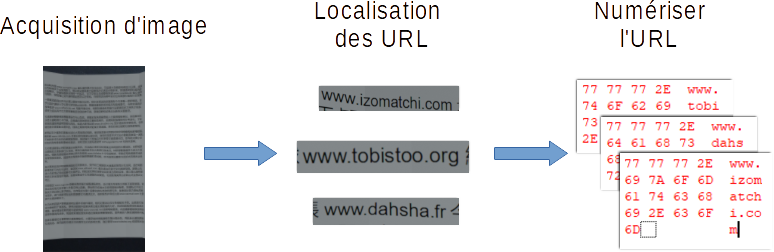
\includegraphics[height=6cm,width=16cm]{Chapitre3/img_2.png}
          \caption{Étapes de numérisation d'une URL.}
          \label{img2}
          \end{figure}

Où: 
\begin{itemize}
\item \textbf{L'acquisition d'image:} Cette phase consiste à obtenir l'image souhaitée qui peut contenir au moins une adresse Web, l'acquisition peut être effectuée à l'aide d'une caméra, téléchargée à partir d'Internet ou chargée à partir d'un disque.
\item \textbf{La localisation de l'URL:} Cette phase joue un rôle crucial dans la localisation des URL dans l'image saisie. Les méthodes de détection d'objets conviennent parfaitement pour accomplir ce processus.
\item \textbf{La numérisation de l'URL:} Cette phase finale prend comme entrée les informations de la boîte englobante (position du point en haut à gauche, largeur et hauteur) et convertit l'URL détectées en une représentation appropriée pour une utilisation dans les recherches en ligne. 
\end{itemize}

Dans ce mémoire, nous nous concentrerons principalement sur la deuxième étape qui est la localisation ou la détection de l'URL dans une image contenant un texte.

La détection d'une URl peut être utile dans plusieurs domaines, particulièrement dans le domaine du tourisme. Le touriste peut prendre une photo d'une URL et afficher les informations du site Web sans avoir à taper sur son clavier. Les propriétaires d'entreprises, de magasins et leurs clients peuvent annoncer et publier des informations en laissant des URL aux services qu'ils proposent sur leurs espaces publicitaires et les utilisateurs peuvent récupérer la ou les URL en cliquant sur un bouton. Le modèle peut également être utilisé pour capturer des références URL tout en écoutant une présentation lors d'une conférence.  Compte tenu de la capacité des appareils photo des téléphones intelligents ces derniers temps, prendre une photo d'une URL en transit devrait donner une image "de bonne qualité" qui peut être transmise en tant qu'entrée à un modèle et la ou les URL d'intérêt seront récupérées.

L'objectif principal de ce mémoire est d'exploiter le domaine de l'apprentissage profond et son application à la détection d'objets. Puis, en utilisant des images contenant des URL comme exemple, le but principal de ce mémoire est d'implémenter et d'évaluer les performances de trois  modèles de référence dans le domaine, à savoir  YOLO3, YOLO4, et YOLO5 pour des images contenant de nombreuses difficultés, en appliquant des techniques de traitement d'images traditionnelles telles que la rotation, et l'ajout de bruit, ...  existants dans les situations réelles.

\section*{Structure du document}
Le mémoire est composé de trois chapitres et une conclusion:

\begin{itemize}
\item Le premier chapitre introduit le domaine de la détection d'objets.
\item Le deuxième chapitre est consacré à la détection d'objets en utilisant les outils de l'apprentissage profond. Il présente les principales techniques qui ont été développées dans ce contexte, ainsi que les principales bases d'images et métriques utilisées pour l'évaluation.
\item Le troisième chapitre décrit les différentes expérimentations, ainsi que les résultats obtenus et leur synthèse.
\item La conclusion conclut le travail réalisé et présente les différentes perspectives.
\end{itemize}